% !TEX root = ../main.tex
\chapter{基于Vision Transformer的深度哈希检索模型}
由于其检索的速度以及较低的内存开销, 深度哈希在大规模图像检索领域获得了广泛的关注。直到本章的算法提出前, 这个领域的所有的深度哈希模型都是基于卷积神经网络而设计, 例如, \textbf{ResNet}~\cite{he2016deep}, \textbf{AlexNet}等。在本章中, 受最近Vision Transformer架构的启发, 我们设计了第一个完全基于Vision Transformer的深度哈希架构来进行大规模的图像检索。具体来说, 我们的架构包含两个基本的模块: (1) 基于Vision Transformer (ViT), 我们设计了一个孪生Vison Transformer的主干架构来进行特征提取。为了学习细粒度的特征, 我们设计了一个双流特征学习的Transformer块来同时学习局部和全局的特征。(2)同时, 我们采取一个基于动态创建的相似度矩阵作为监督标签设计的贝叶斯学习框架来学习相似度保持的紧凑的二进制哈希编码。整个框架是通过一种端到端的方法同一训练。据我们所知, 本章提出的深度哈希框架是第一个完全不基于卷积神经网络的深度哈希学习框架。本章的算法在三个被广泛研究的标准数据集上进行全方面的测试, 数据集包括:~\textbf{CIFAR-10},~\textbf{NUSWIDE},~和~\textbf{IMAGENET}。数据结果证实了我们的方法和现阶段的先进的深度哈希算法比较具有极高的性能的优越性。在三个数据集上, 我们比较第二优越的算法分别获得了 $8.2\%$, $2.6 \%$和$12.7\%$的性能增长。

\section{引言}
近些年来, 由于互联网技术的普及, 以及计算机技术, 便携摄像的进步, 传感器技术, 云计算以及各种社交网络的兴起, 由无数终端用户生成的视频和图片数据以爆炸性的速度增长。如何对海量的数据进行检索是利用数据进行其他大规模商业应用的基石, 因此准确和高效进行数据检索的研究开始受到学术界和工业界研究人员的大规模的关注。在这些技术研究中, 大规模图像检索由于其广泛的工业界应用, 如推荐系统, 搜索引擎, 遥感检索系统等, 受到了日益增长的关注。 在所有解决这一具有挑战性的任务的方法中\cite{fu2017fast, ge2013optimized, jegou2010product, malkov2018efficient}, 基于二进制码的哈希方法取得了令人瞩目的成果。基于哈希的方法通过学习一个哈希函数, 将高维像素空间中的图片映射到低维的二进制汉明空间中, 其中在低维度的汉明空间的图片对应的哈希码需要保存原图片之间的视觉相似性。过去的这些你那, 一大批的基于哈希的方法被提出。 根据它们提取特征的方法, 我们可以将其简单的分成两个类别: (1) 基于手工特征提取的方法 (2) 基于深度学习的方法。\par

\begin{figure}[!htp]
    \centering
    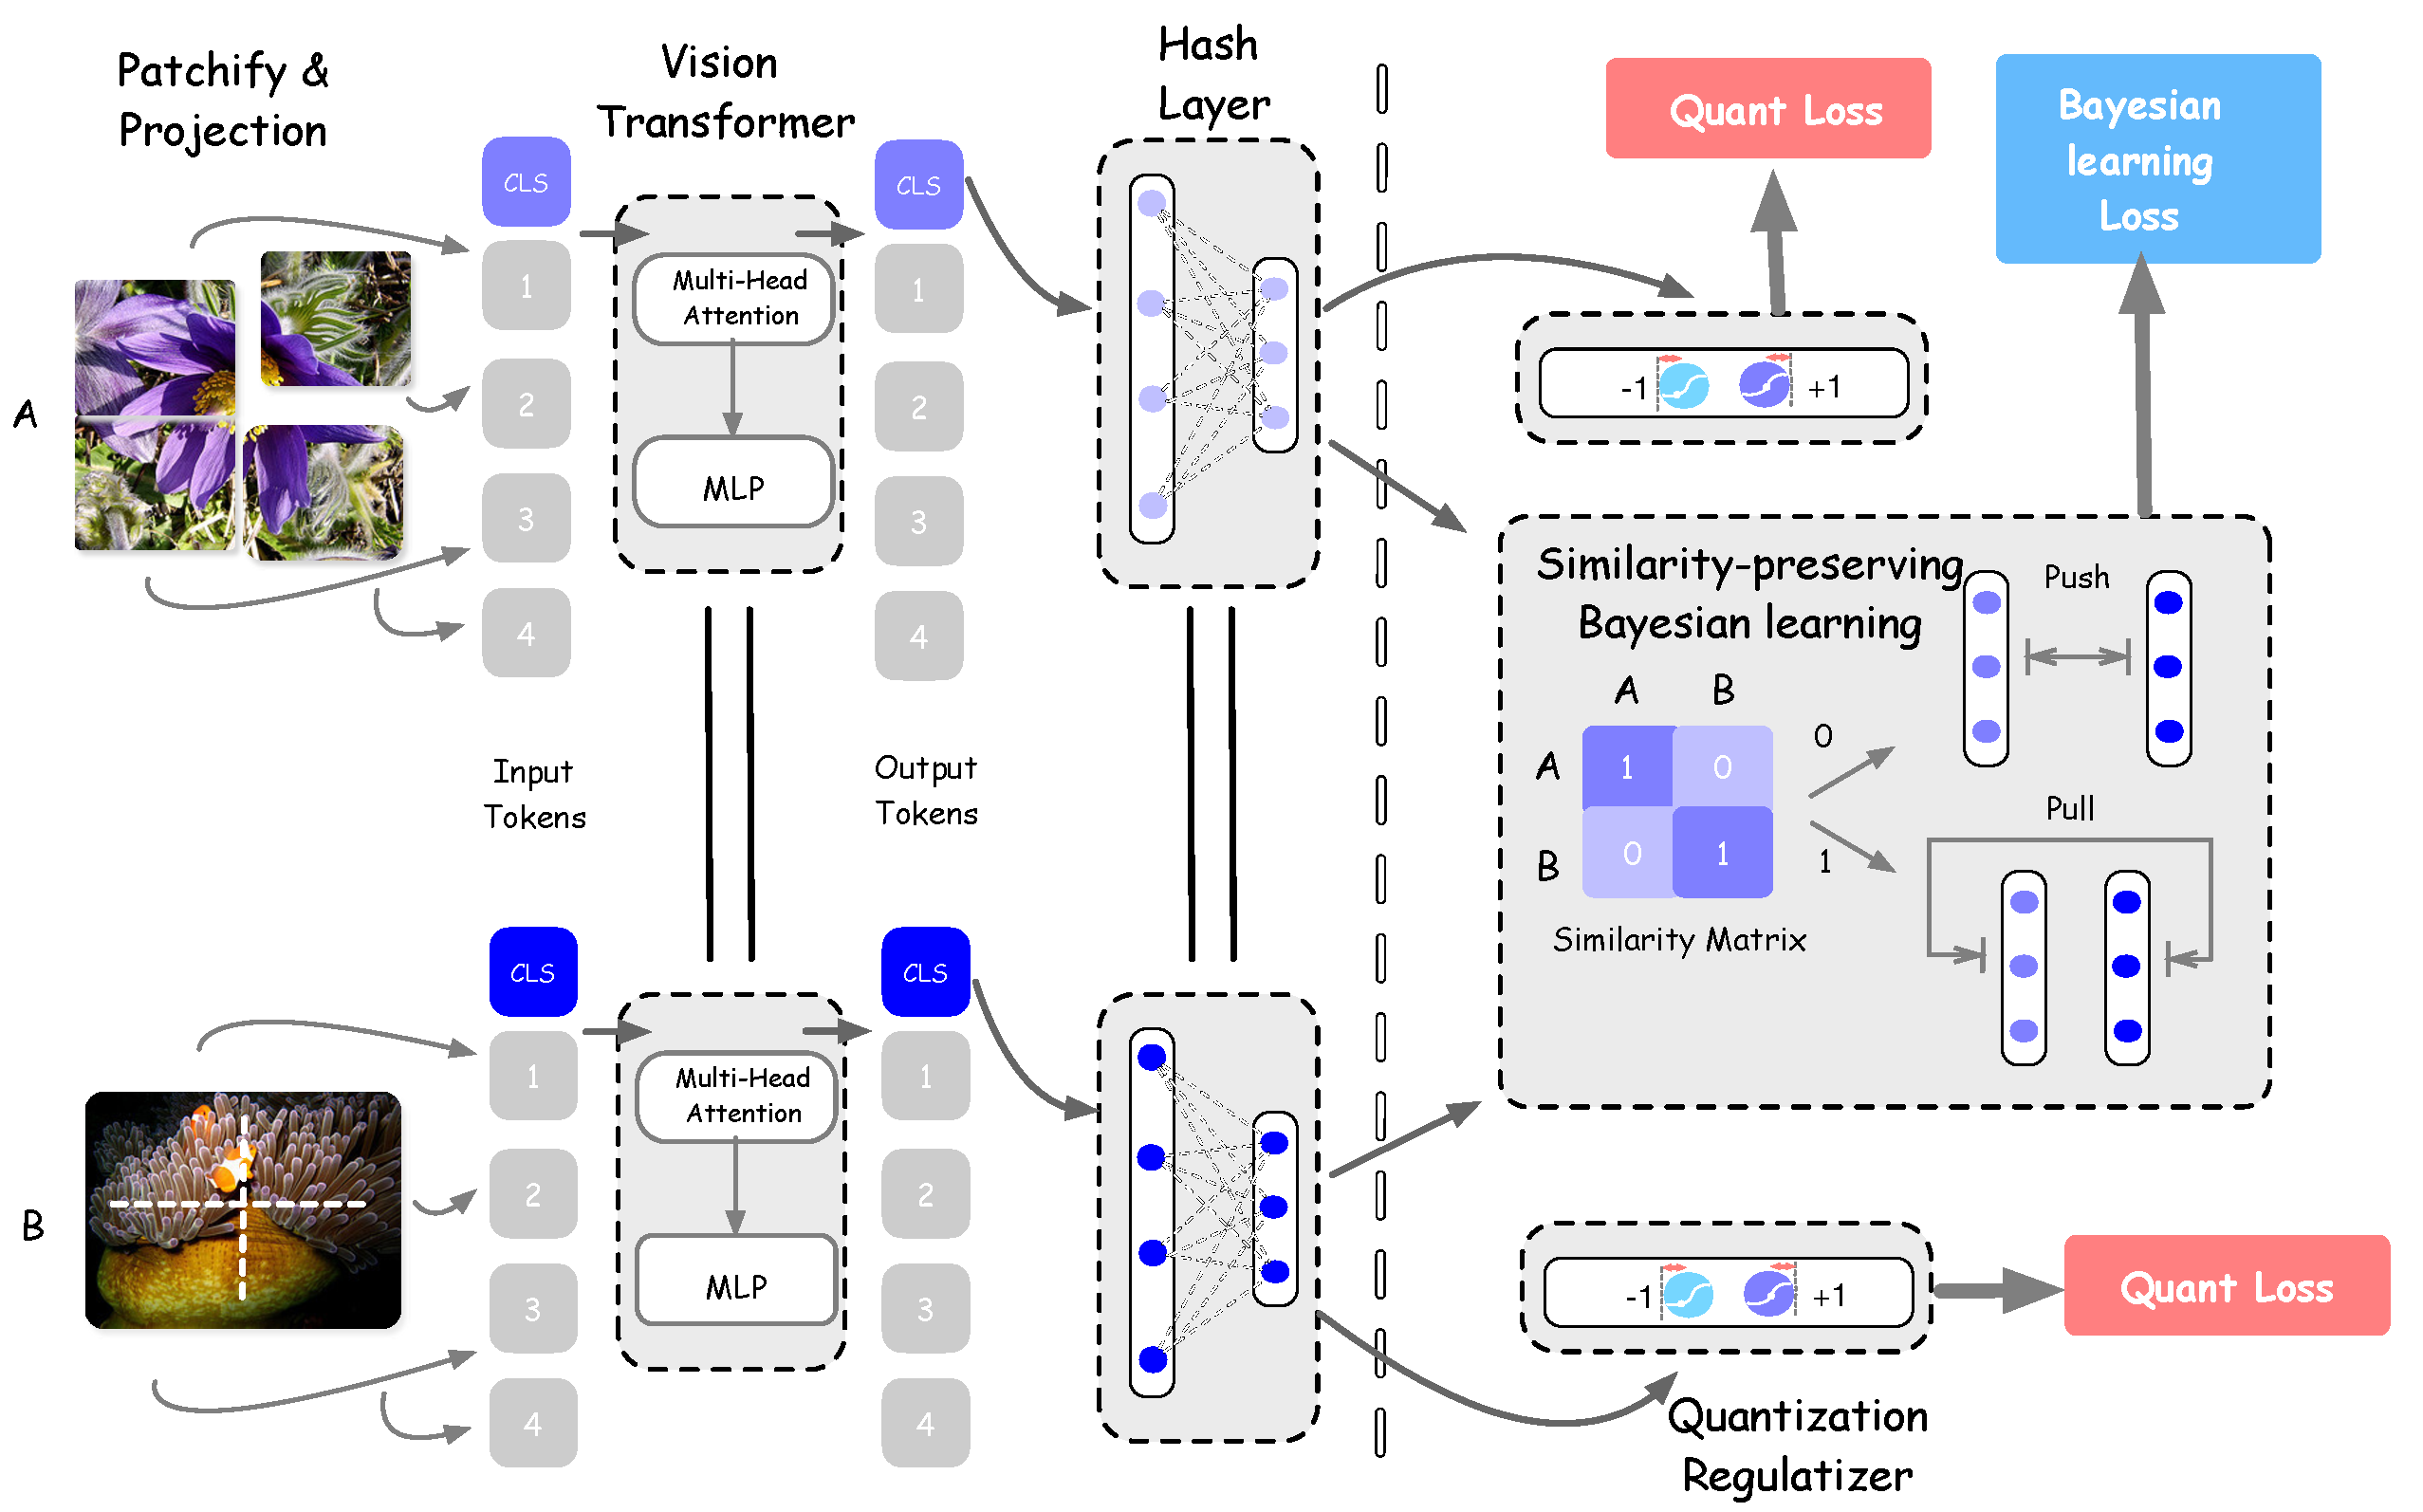
\includegraphics[width=15cm]{04/subfig.pdf} \\
    \bicaption[基于孪生Vision Transformer的图片检索基本框架]
      {对于一个图片对 (A, B), 我们将它们分割成固定大小的多个小图片块。然后将每个小块的像素转变成一个向量并且通过全连接将维成为一系列的嵌入表示。随后, 我们在这一系列的嵌入表征前添加一个随机初始化的向量作为分类嵌入。随后两串表征被输入进孪生Transformer模型并且通过一个哈希层生成$B$为的哈希向量。我们使用基于贝叶斯的学习框架来进行相似度保持学习。}
      {For an image pair (A,B), we cut them into several patches. Then every patch is flattened and projected to a fix-sized embedding with a fully connected layer, resulting in a sequence of embeddings. Subsequently, we add a classification token in the front of each sequence. Then, two sequences are fed into the Siamese transformer architecture. At last, we add a hash layer projecting the feature into B-bit hash vectors. The Bayesian learning module is employed to preserve the similarity in the \textit{Hamming} space for each pair. }
   \label{fig:subfig}
\end{figure} 

基于手工特征的浅层次哈希方法一般是通过基于人工设计的视觉特征描述符来进行哈希函数的学习~\cite{charikar2002similarity, indyk1997locality, weiss2008spectral}, 例如 \textbf{GIST}~\cite{oliva2001modeling}等。经典的浅层次哈希方法有~\textbf{LSH}~\cite{indyk1997locality}, 其主要思想是将相似的高维数据以比较大的概率被映射到相近的哈希编码中。然而由于基于手工提取的特征向量其实并不能准确的刻画保存原图片的有区别性的信息, 这导致了基于手工特征的哈希算法有一道无法逾越的性能鸿沟。为了减轻这个问题的影响, 随着AlexNet~\cite{}的提出, 基于深度学习的特征提取方法开始成为计算机视觉领域的主流。基于深度学习的模型~\cite{dosovitskiy2020image, russakovsky2015imagenet}相比较基于手工特征的方法通常而言可以获得显著的性能提升。基于深度学习的哈希学习方法一般包含两个阶段。 第一阶段致力于基于深度卷积神经网络, 例如 \textbf{AlexNet}等, 学习有判别性的特征。第二阶段包含包含设计各种非线性的函数来将连续性的神经网络输出转化成固定的哈希长度的二进制哈希码, 并且通过各种度量学习的损失函数~\cite{cakir2019hashing,cao2018deep,erin2015deep,gong2012iterative, li2015feature}来在汉明空间保存其对应的图片的视觉相似性。 \par
最近, Transformer~\cite{vaswani2017attention}模型展示了其在自然语言领域的卓越性能~\cite{brown2020language, devlin2018bert}。随后, Google设计了 Vision Transformer~\cite{dosovitskiy2020image}, 一种基于 Transformer的变种, 正式将Transformer引入进计算机视觉领域。Vision Transformer 开始在各个计算机视觉任务上超越传统基于卷积神经网络的模型(例如, 图像分类~\cite{dosovitskiy2020image}, 行人重识别~\cite{he2021transreid},等)。如图~\ref{fig:subfig}所示, Vision Transformer 通过首先将输入的图片分割成一系列的2D图片块。 随后, 将图片块转换成向量并且通过可以学习的转换矩阵来将向量将维度成低维度的特征表示。 随后, 一系列的输入向量可以被输入进标准的Transformer的编码器架构来学习特征表示。受Vision Transformer的高性能表现的启发, 我们思考完全基于Vision Transformer设计一个深度哈希框架的可行性。\par
在本章中, 我们基于Transformer 设计了一个新型的深度哈希框架-\textbf{TransHash}, 这是有史以来第一个不基于卷积神经网络作为主干网络来进行特征学习的深度哈希架构。具体而言, 为了进行成对的哈希学习, 我们设计了一个孪生多粒度Vision Transformer主干网络 (Multi-Granular Vision Transformer, MGVT)。它包含了两个完全一致的多粒度学习的Transformer网络, 并且这两个网络是完全共享所有参数~\cite{bromley1993signature}。具体而言, 为了进行多粒度的学习, 我们受\textbf{TransReID}~\cite{he2021transreid}所启发, 我们在传统的Vision Transformer的最后一层上设计了一个双流特征学习机制, 将最后一个Transformer块设计成两个并行的分支。对于第一个分支, 它是用来进行全局特征的学习。对于并行的第二个分支, 我们将前一个Transformer块的输出序列进行重新分组成$K$个序列组。
